\documentclass[../Main.tex]{subfiles}

\begin{document}

\begin{tcolorbox}[colback=light-orange, boxrule=0pt]
  \begin{multicols}{3}
    \textcolor{blue}{\textbf{ABSTRACT:}}
Pythoplankton blooms in the Baltic Sea are an annual event in the Batlic. They usually occur in the spring and fall of the year.
    Because of their great ecological impact, phytoplankton blooms are often the focus of research projects. Using satellite imagery and water samples, effects of physical parameters have been studied on phytoplankton growth. Physical parameters have mostly been limited to temperature, light and density.
The lack of precision and continuity of the collected data often made it challenging to find correlations.
   Here we show an overview of a new high-resolution dataset taken by glider in the Baltic Sea from March to October 2021.
    The data provide insight into two phytoplankton blooms that occurred from mid-March to April and from mid-May to early July.
It was found that the blooms do not depend on the same physical drivers. 
Phytoplankton blooms can be caused by different factors that influence to a large extent the distribution of phytoplankton in the water stratification. 
   The results show that it is possible to find relationships between different physical drivers of phytoplankton blooms when analyzing high resolution and continuous data. Hereby gliders are bleeding edge vehicles to data collection.
\ \\
\ \\
    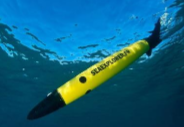
\includegraphics[width=0.33\textwidth]{Glider.png}
 \end{multicols}
\end{tcolorbox}
\end{document}
